\documentclass{standalone}

\usepackage{ tikz }
\usetikzlibrary{automata, positioning, arrows}

\begin{document}
    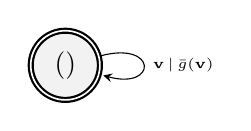
\begin{tikzpicture}[->, >=stealth, node distance=3cm, every state/.style={thick, fill=gray!10}, initial text=$ $, every edge/.append style={font=\tiny}]
        \node[state, accepting] (s) {$()$};

        \draw (s) edge [loop right] node{$\textbf{v} \,|\, \bar{g}(\textbf{v})$} (s)
        ;
    \end{tikzpicture}
\end{document}